\chapter{Speaker measurement}
To compare the MATLAB model with a real speaker, several measurements have been carried out using a PC, the Argon DA-1 amplifier, the Behringer Xenyx 302USB mixer (for PC to microphone connection), a Behringer ECM8000 microphone and alternating between the two speakers shown in \cref{fig:measspeak}.

\begin{figure}
	\centering
	\begin{subfigure}{.5\textwidth}
		\centering
		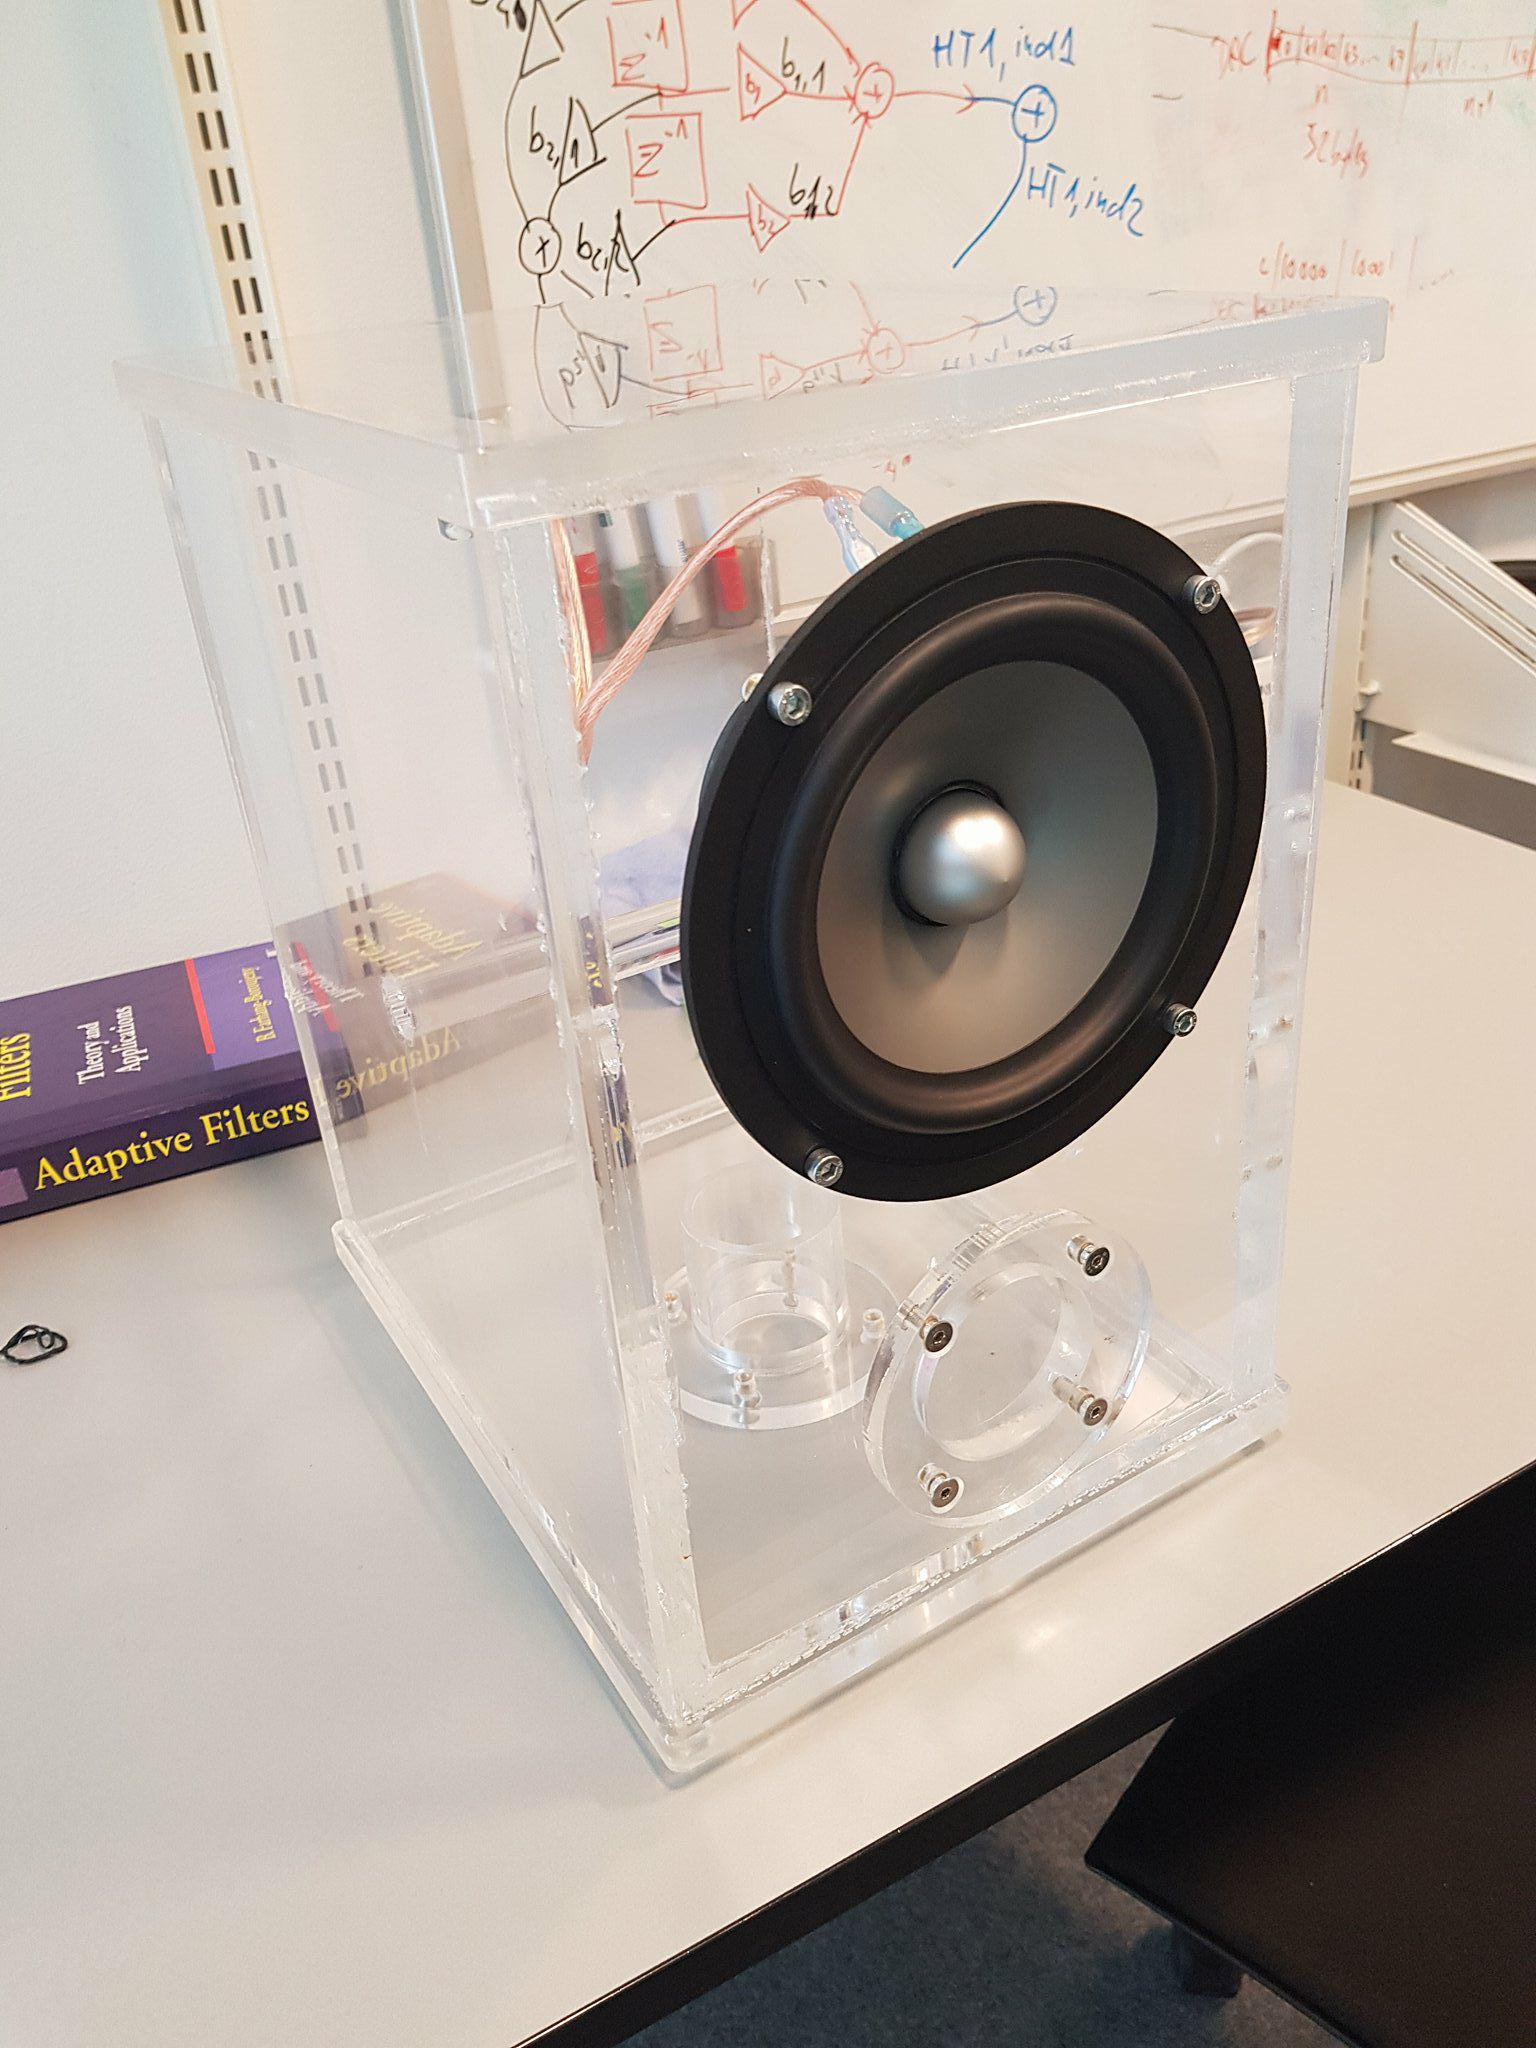
\includegraphics[width=.9\linewidth, clip, trim={0 6cm 0 6cm}]{gfx/Speaker_plexi.jpg}
		\caption{A see-through speaker with the possibility to remove or insert bass reflexes. Approximate volume: \SI{18}{\litre}. Drive Unit: Fountek FW168.}
		\label{fig:measspeak1}
	\end{subfigure}%
	\begin{subfigure}{.5\textwidth}
		\centering
		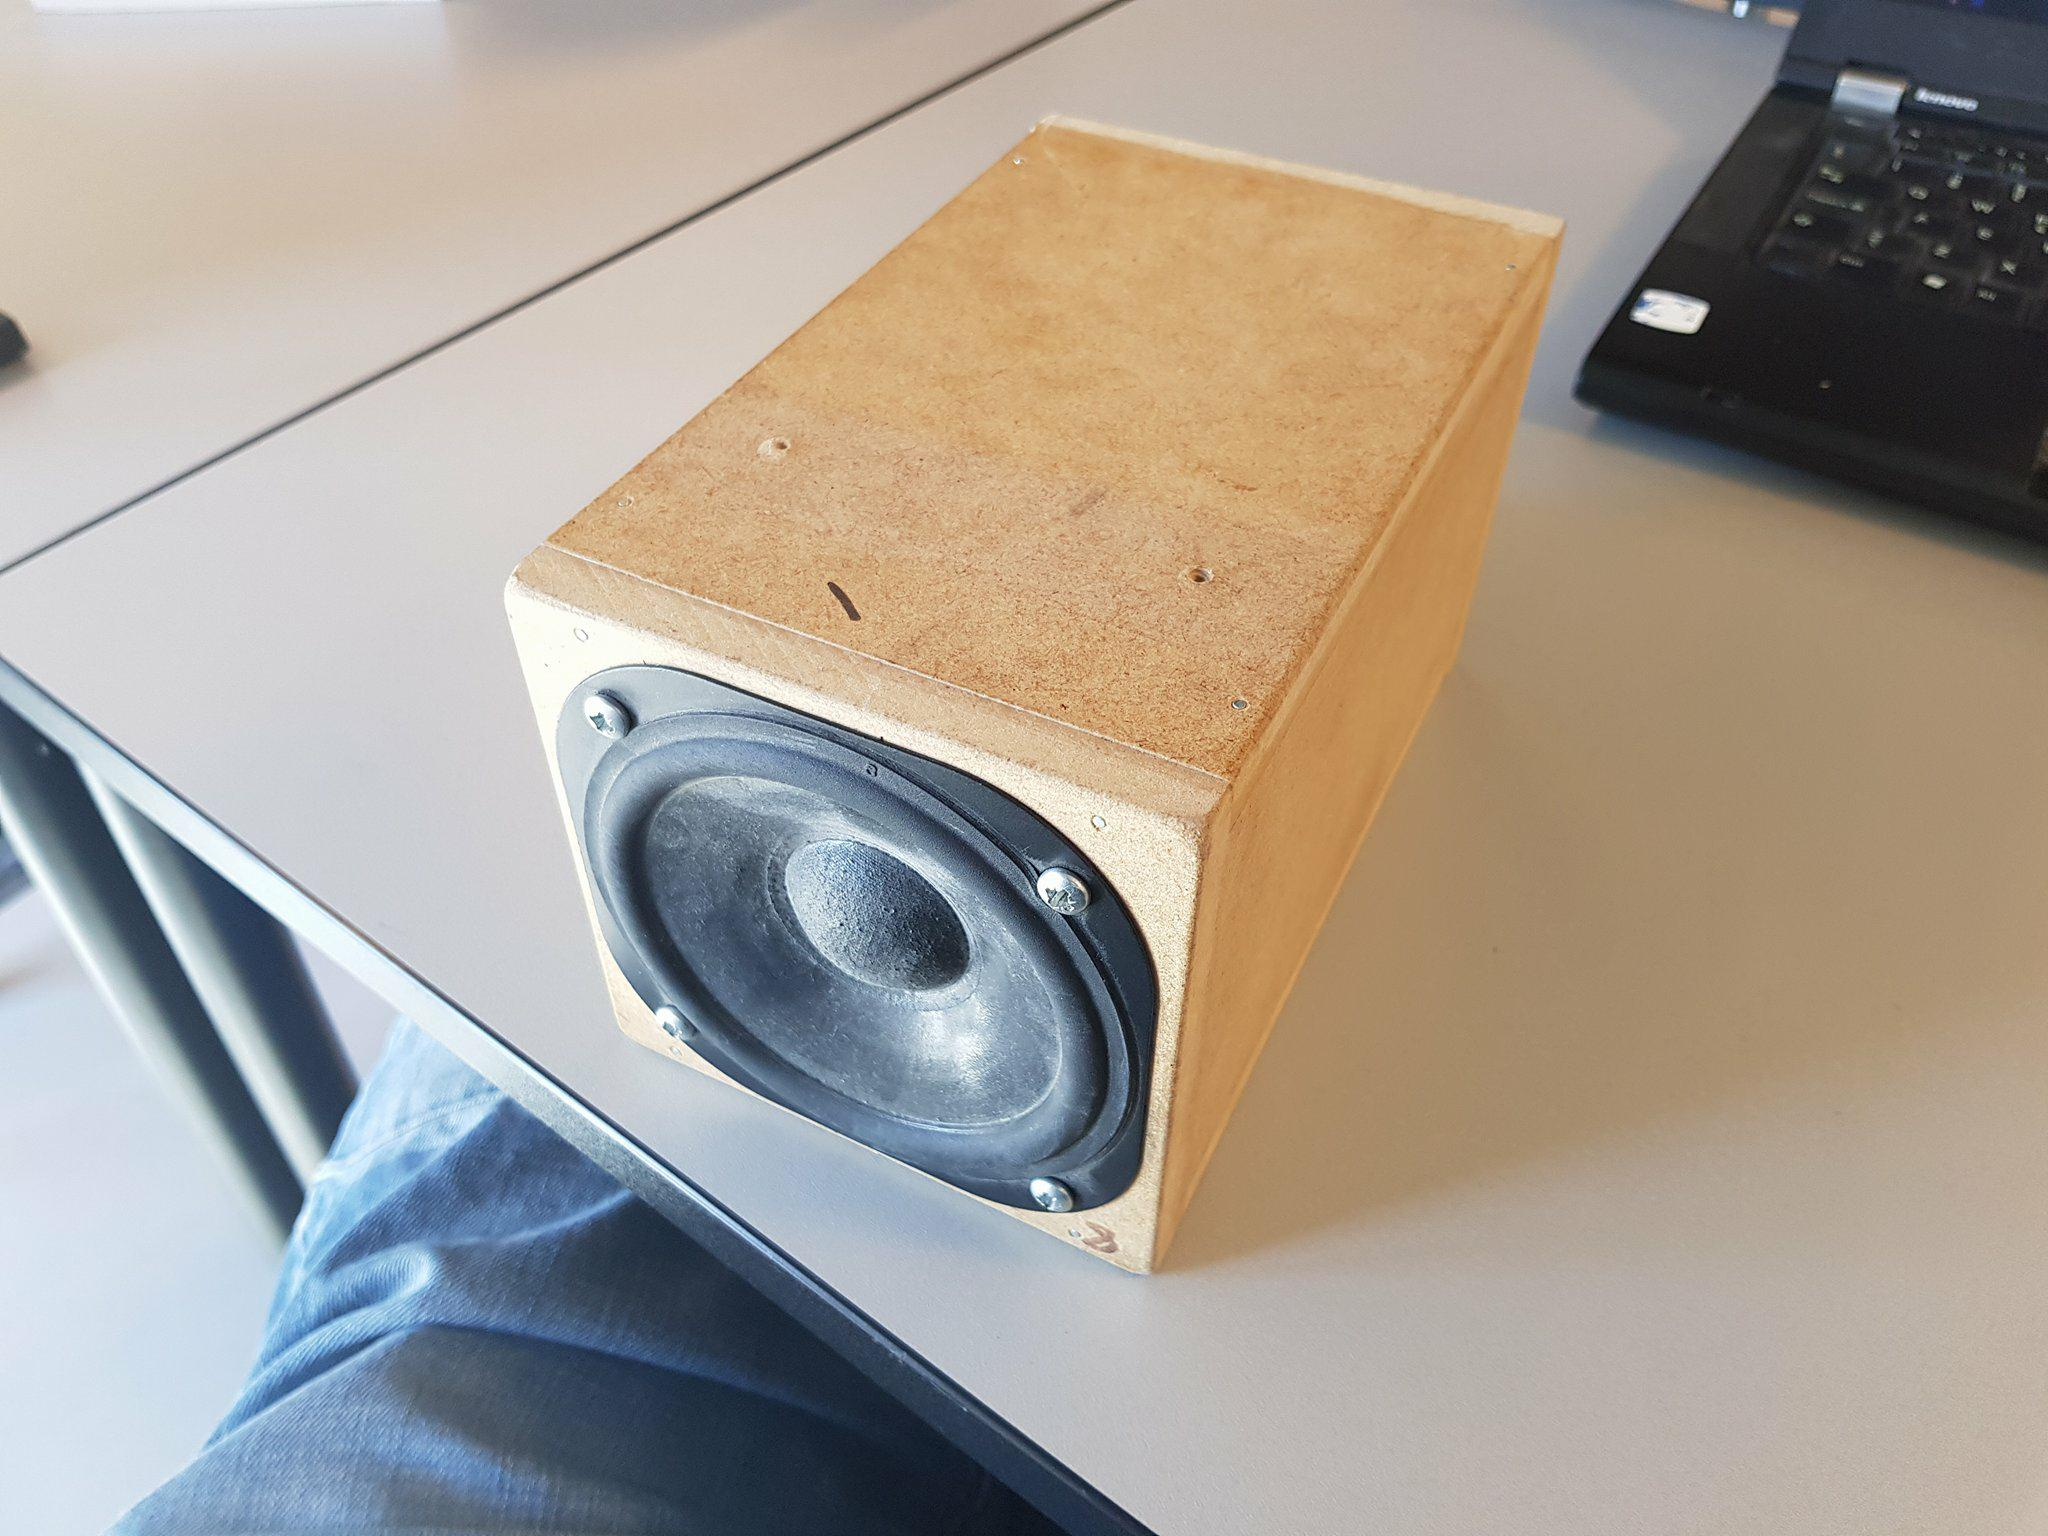
\includegraphics[width=.9\linewidth, clip, trim={17cm 3cm 14cm 0}]{gfx/Speaker_wood.jpg}
		\caption{Wooden speaker. Approximate volume: \SI{1.5}{\litre}. Drive Unit: Vifa C11WG-09.}
		\label{fig:measspeak2}
	\end{subfigure}
	\caption{The two speakers used for measurements.}
	\label{fig:measspeak}
\end{figure}

%% !TEX root = ../../main.tex
% !TEX spellcheck = en_GB
\section{Analysis}
The framework must include a speaker comprising of a Drive Unit and a closed cabinet, should include a crossover filter and could include a bass reflex, according to \nameref{sec:delimitations}.
The frequency response of each unit should be exposed 
for investigation and the frequency response of the entire system should be available.
%% !TEX root = ../../main.tex
% !TEX spellcheck = en_GB
\section{Design}
The design of the MATLAB framework is shown in \cref{fig:classbdd}.

\paragraph{The TransferFunction class} implements the \mintinline{matlab}{plotResponse(f)} method, and the  abstract method \mintinline{matlab}{transform(x)}.
\mintinline{matlab}{plotResponse(f)} plots the amplitude spectrum in the range given by the argument \mintinline{matlab}{f}.
It uses the implemented, by any subclass, \mintinline{matlab}{transform(x)} method to access the frequency response.

\begin{figure}
	\centering
	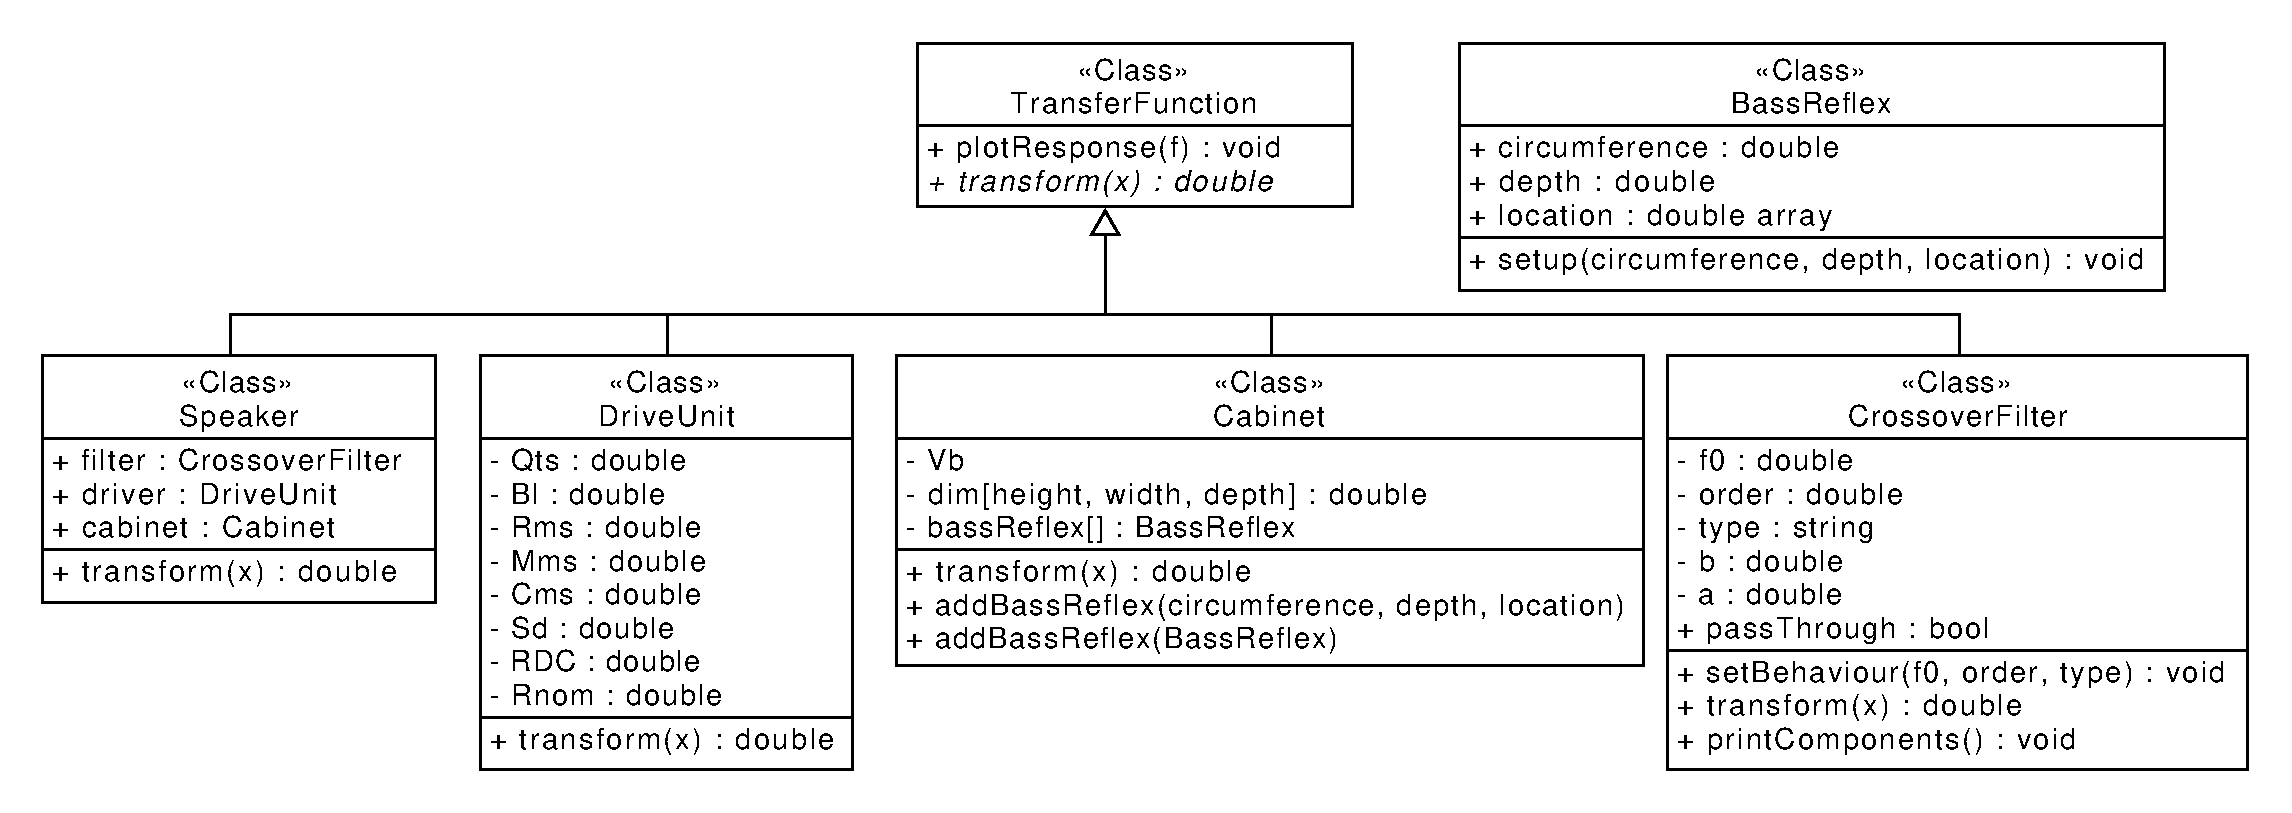
\includegraphics[width=\linewidth]{gfx/Design/Class_BDD}
	\caption{Class diagram of the MATLAB framework.}
	\label{fig:classbdd}
\end{figure}

\paragraph{The Speaker class} contains the objects necessary to calculate the transfer function for the complete speaker.
It's purpose is to collect the other units, to test them together, and to provide the frequency response to compare with the measured response.

\paragraph{The DriveUnit class} describes the drive unit on the basis of Thiele/Small parameters\cite{thielesmall} and \cref{eq:transdriveunit} \cite[p.~41]{Elektroakustik}.
The \mintinline{matlab}{plotResponse(f)} function plots the response of the drive unit in an infinite baffle.\fxnote{Infinite baffel or infinite closed box?}

\begin{equation}
	p = \frac{\rho S_D B l U_G}{2\pi r M_{MS} R_E}\left|\frac{s^2}{s^2 + \frac{\omega_s}{Q_{TS}}s+\omega_s^2}\right|
	\label{eq:transdriveunit}
\end{equation}

\paragraph{The Cabinet class} describes a closed box cabinet, with the possibility to add a number of bass reflexes and check if their locations are valid.

\paragraph{The CrossoverFilter class} is meant to filter the input before it reaches the physical parts of the speaker.
It is meant to either be used to filter the signal in an appropriate way if several drive units are installed, or to try to refine the signal, if the speaker response is not satisfactory.

\paragraph{The BassReflex class} is a bass reflex tube placed somewhere on the cabinet.
% !TEX root = ../../main.tex
% !TEX spellcheck = en_GB
\section{Implementation}
\fxnote{Possibly example of a class and description of it. Mostly ref to appendix for code. Example of output, maybe compared to other output.}
The \mintinline{matlab}{DriveUnit} class is shown below for clarification. 
The overall structure is a standard Matlab class inheriting from TransferFunctions, as shown in \cref{fig:classbdd}. 
Following are the private and public properties and the public methods, including the implementation of the \mintinline{matlab}{transform(f)} method.

Matlab evaluates the property definition section only once and assigns the same value to the property of every instance in the class.\fxnote{https://se.mathworks.com/help/matlab/matlab\_oop/specifying-properties.html}
The default values are specified individually as private or public.
The private properties include constants so these properties gets a default value that other instances can not access. 
Instead the datasheet values for the drive unit is public so other instances, e.g. \mintinline{matlab}{Cabinet}, can access these values.

The implementations of all the classes in the MATLAB framework can be found in appendix \ref{app:code}. 


\begin{minted}[linenos, breaklines, bgcolor=lightgray]{matlab}
classdef DriveUnit < TransferFunctions
    properties (Access = private)
	%% Defaults
	% Density of air (kg/m^3)
	rho     = 1.1839;
	% Distance to microphone (m)
	R      = 1;
	end
    properties (Access = public)
	%% Data sheet values
	fs
	Qts
	Bl
	Rms
	Mms
	Cms
	Sd
	Re
	Rnom
	%% Derived values
	UG
    end
\end{minted}

The methods are public so \mintinline{matlab}{TransferFunctions} can access the \mintinline{matlab}{transform(f)} method to plot the frequency response of the drive unit. See appendix in \cref{app:code} for implemtation of \mintinline{matlab}{TransferFunctions}.
The implementation of the \mintinline{matlab}{transform(f)} method create the transfer function for a drive unit using the properties specified.
The transfer function for a drive unit can be found in \cref{seq:driveunit}, \cref{eq:dutfclosed}.

\begin{minted}[linenos, breaklines, firstnumber=last, bgcolor=lightgray]{matlab}
    methods (Access = public)
	function p = transform(obj, f)
	    % Create the transfer function for a drive unit
	    % mounted in an infinite sealed enclosure.
	    setDerivedParameters(obj);
	    s = 1i .* 2 .* pi .* f;
	    k0 = (obj.rho * obj.Bl * obj.Sd * obj.UG) / (2 * pi * obj.R * obj.Re * obj.Mms);
	    k1 = ((obj.Bl^2) / (obj.Re * obj.Mms)) + (obj.Rms / obj.Mms);
	    k2 = 1 / (obj.Mms * obj.Cms);
	    p = k0 .* (s.^2 ./ (s.^2 + s .* k1 + k2));
	end
\end{minted}

The \mintinline{matlab}{setParameters(Qts, Bl, Rms, Mms, Cms, Sd, Re, Rnom, fs)} 
\newline method is used to set the parameters for the drive unit.
The Thiele/Small parameters is found in the datasheet for the given drive unit. 
A input validation is performed for the Sd parameter as it is specified either in $\si{\square\meter}$ or $\si{\square\centi\meter}$ in the datasheets.
\begin{minted}[linenos, breaklines, firstnumber=last, bgcolor=lightgray]{matlab}
	function setParameters(obj, Qts, Bl, Rms, Mms, Cms, Sd, Re, Rnom, fs)
	    % Sets the parameters for the drive unit.
	    % The parameters should be found in the datasheet
	    % for the given drive unit. 
	    if  (Sd > 1) && (Sd < 1000)
		obj.Sd = Sd/1000;
	    else
		warning('Sd is specified in cm^2')
	    end
	    obj.Qts = Qts;
	    obj.Bl = Bl;
	    obj.Rms = Rms;
	    obj.Mms = Mms;
	    obj.Cms = Cms;
	    obj.Re = Re;
	    obj.Rnom = Rnom;
	    obj.fs = fs;
	    setDerivedParameters(obj);
	end
\end{minted}

The \mintinline{matlab}{setDerivedParameters()} method sets the $U_G$ voltage given on the nominel resistance $R_{nom}$ specified in the \mintinline{matlab}{setParameters} method. 
The $U_G$ voltage is set so the input for the drive unit is \SI{1}{\watt} since the sensitivity is specified in \si{\decibel} per \SI{1}{\watt} in a distance of \SI{1}{\meter}.
\begin{minted}[linenos, breaklines, firstnumber=last, bgcolor=lightgray]{matlab}
	function setDerivedParameters(obj)
	    % Sets the derived parameters 
	    % dependent on the given drive unit.
	    % UG Voltage for 1 W electric power in nominel resistance ohm
	    obj.UG = sqrt(1*obj.Rnom);
	end
\end{minted}

The \mintinline{matlab}{setConstants()} method make it possible for the user to change parameters who usually are constants as density of air. 
If the method is not called the default values specified in the property definition section is applied.   
\begin{minted}[linenos, breaklines, firstnumber=last, bgcolor=lightgray]{matlab}
	function setConstants(obj, rho, R)
	    % Change default values of rho, pRef and R.	
	    % Check for correct number of input arguments
	    if ~(any([1, 3] == nargin))
		error(' Call setConstants(rho, r) with 2 parameters or\n%s',...
		'with 0, setConstants(), to reset to default.');
	    end
	    if nargin == 1
		obj.rho = 1.1839;
		obj.R = 1;
	    else
		obj.rho = rho;
		obj.R = R;
	    end
	end
    end
end
\end{minted}

An instance of the \mintinline{matlab}{DriveUnit} is created and the parameters of the Fountek FW168 drive unit is set with the method \mintinline{matlab}{setParameters()}.
The method \mintinline{matlab}{plotResponse(logspace(1,4,1000))} from the \mintinline{matlab}{TransferFunctions} class plots the response between \SI{10}{\hertz} and \SI{10}{\kilo\hertz}.
In \cref{fig:simdriveunit} the simulated frequency response of the Fountek FW168 drive unit placed in an infinite sealed enclosure is seen.
\begin{minted}[linenos, breaklines, bgcolor=lightgray]{matlab}
k = DriveUnit();
% setParameters(Qts, Bl, Rms, Mms, Cms, Sd, Re, Rnom, fs)
k.setParameters(0.397, 8.2, 1.3036, 14.7e-3, 0.821e-3, 119, 7.2, 8, 45); 
k.plotResponse(logspace(1,4,1000));
\end{minted}

An instance of the \mintinline{matlab}{Cabinet} is created with the volume of the cabinet as an argument.
The Fountek FW168 drive unit is set with the method \mintinline{matlab}{setDriveUnit()}.
The method \mintinline{matlab}{plotResponse(logspace(1,4,1000))} from the \mintinline{matlab}{TransferFunctions} class plots the response between \SI{10}{\hertz} and \SI{10}{\kilo\hertz}.
In \cref{fig:simcabinet} the simulated frequency response of the Fountek FW168 drive unit placed in an cabinet with a volume of \SI{17.9}{\liter} is seen. 

\begin{minted}[linenos, breaklines, bgcolor=lightgray]{matlab}
% 26.8cm x 20.2cm x 33.0cm
V = (26.8e-2*20.2e-2*33.0e-2); 
u = Cabinet(V);
u.setDriveUnit(k);
u.plotResponse(logspace(1,4,100));
\end{minted}

%\FloatBarrier

\begin{figure}[H]
	\centering
	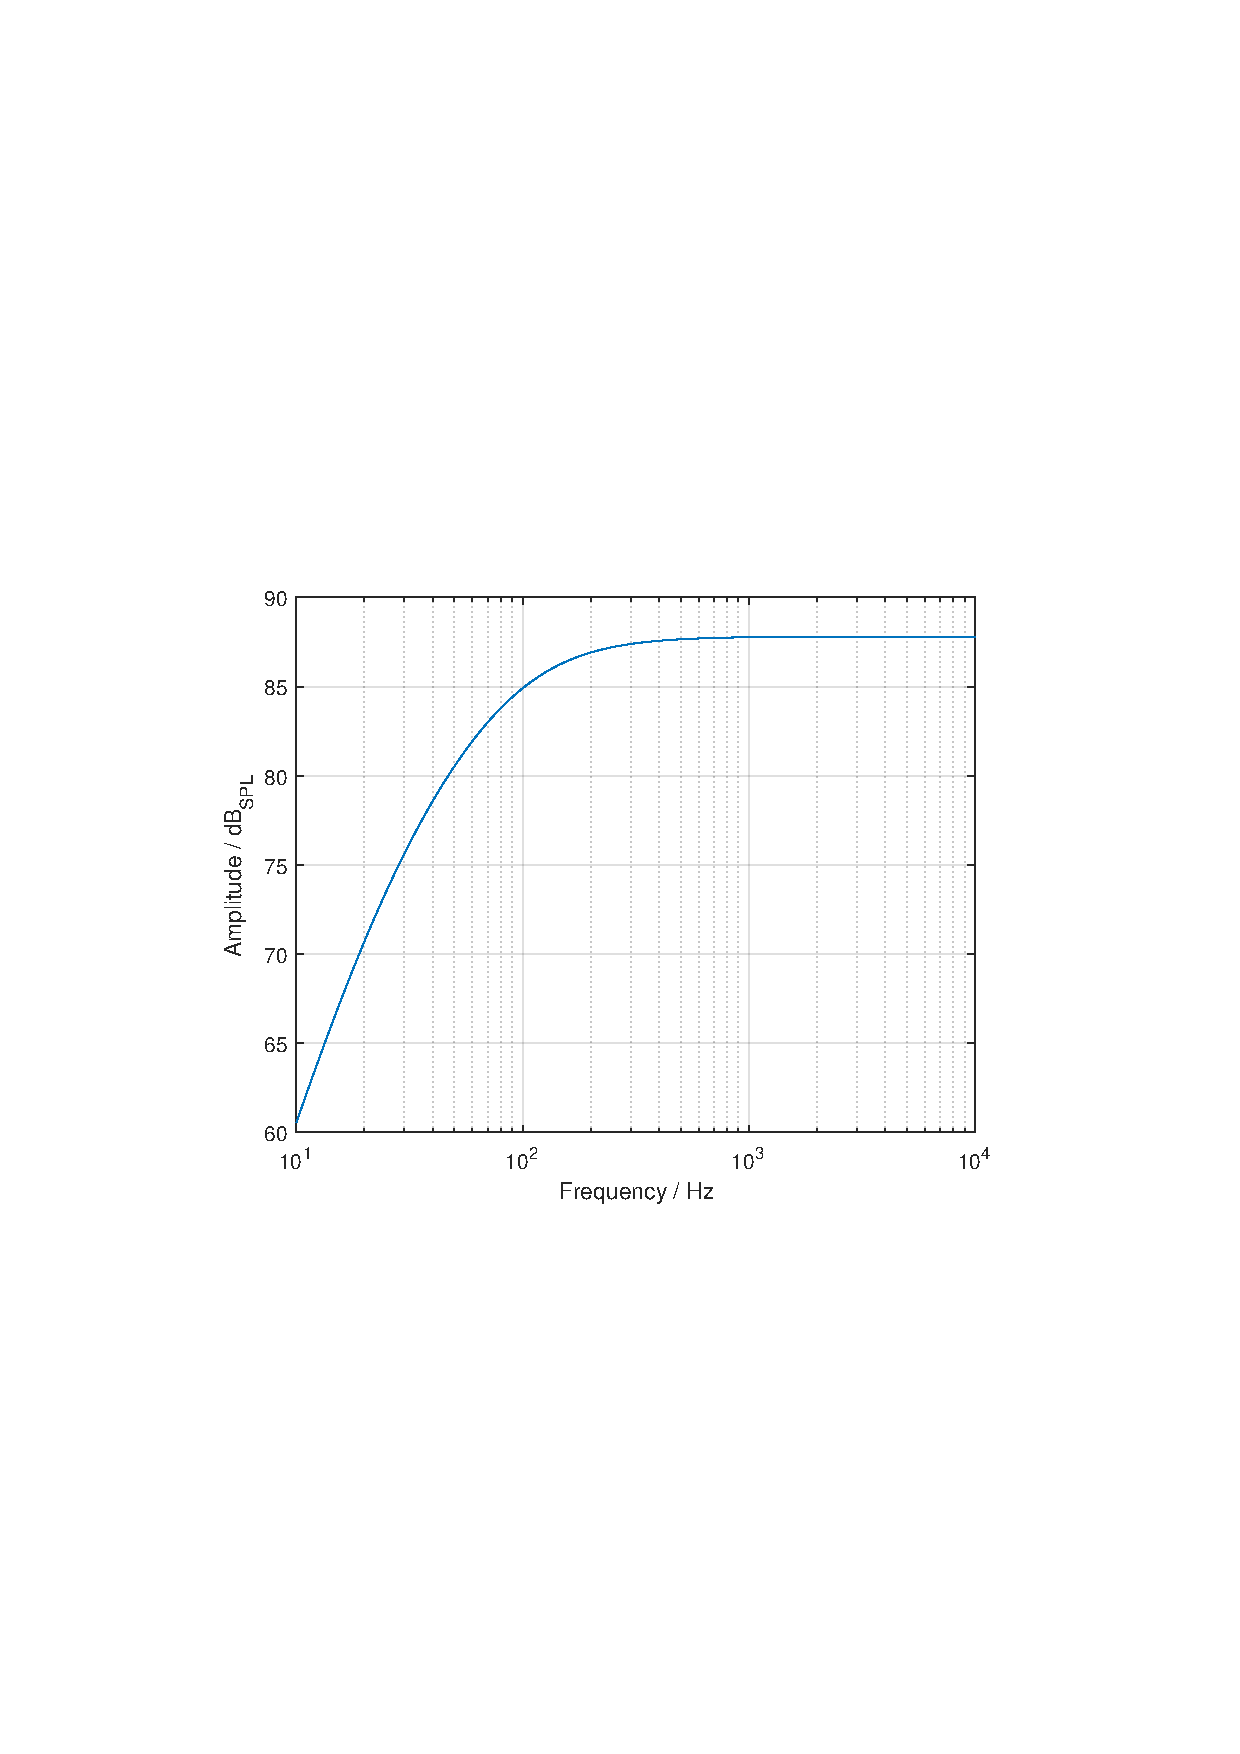
\includegraphics[width=.7\linewidth, clip, trim={3.6cm 8.6cm 4.1cm 10cm}]{gfx/Simulation/DriveUnitSimulation}
	\caption{Simulated output of the FW168 Fountek drive unit.}
	\label{fig:simdriveunit}
\end{figure}

\begin{figure}[H]
	\centering
	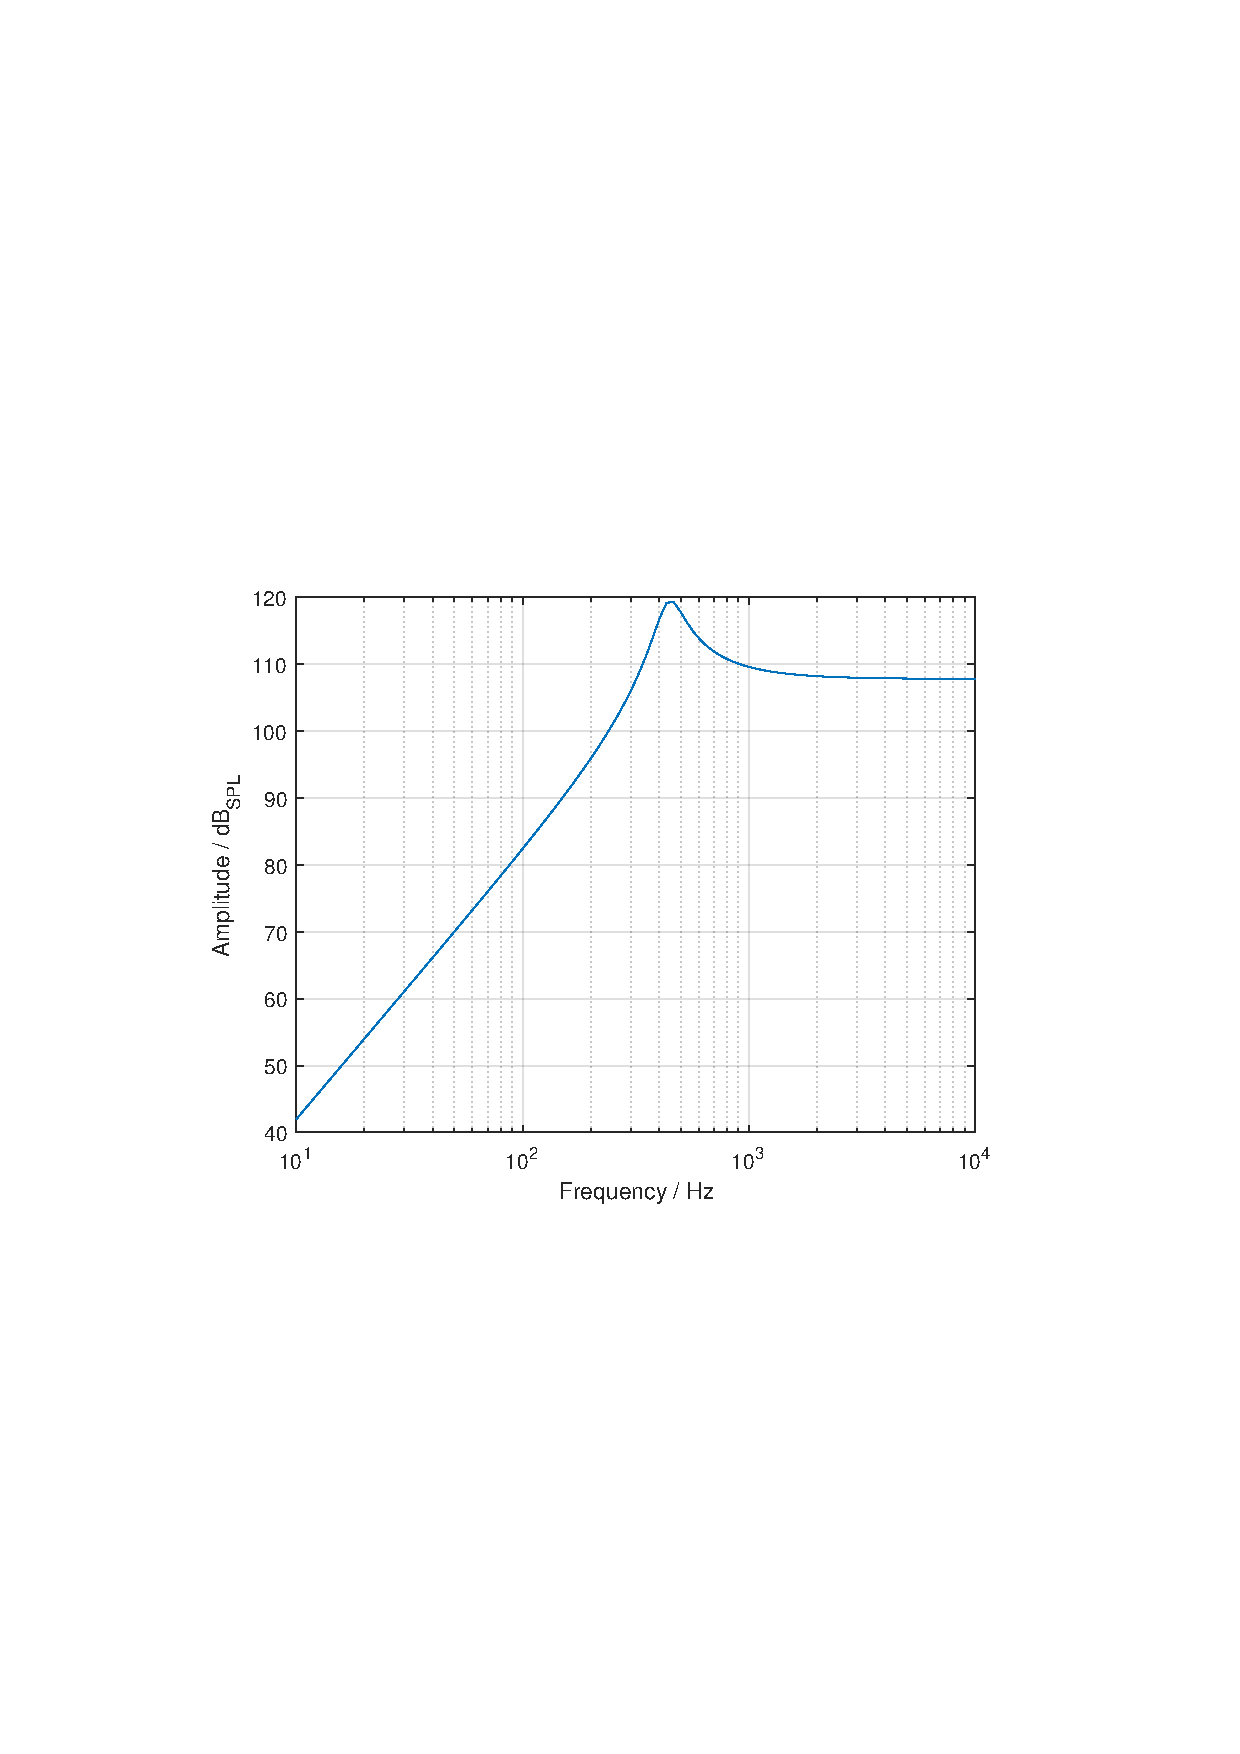
\includegraphics[width=.7\linewidth,, clip, trim={3.6cm 8.6cm 4.1cm 10cm}]{gfx/Simulation/CabinetSimulation}
	\caption{Simulated output of the FW168 Fountek drive unit placed in a cabinet.}
	\label{fig:simcabinet}
\end{figure}

%\FloatBarrier
\section{Measurement}
Three measurements were made with the see-through speaker; closed box, bottom-hole open and bottom \SI{0.27}{\litre} bass reflex. One closed box measurement was made with the wooden speaker. The results are shown in \cref{fig:measAll}.

\begin{figure}
	\centering
	\begin{subfigure}{.5\textwidth}
		\centering
		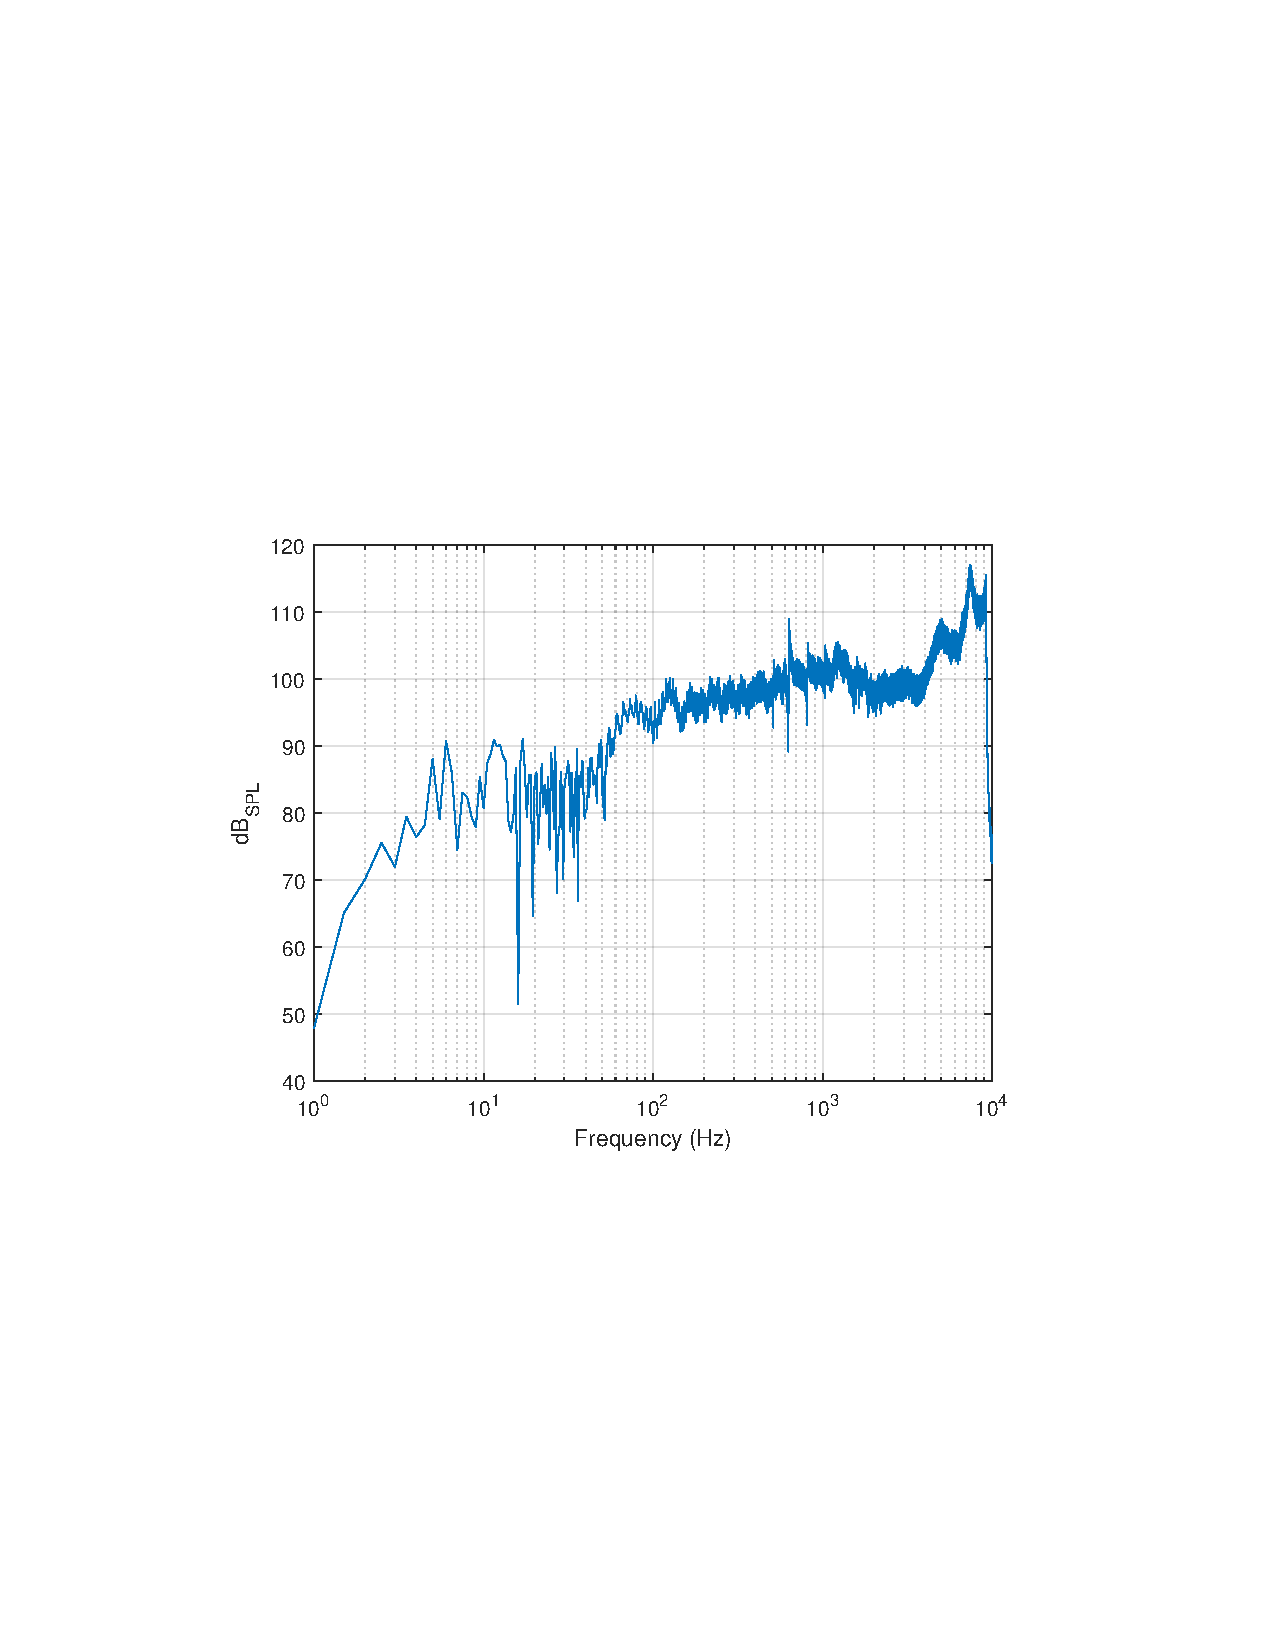
\includegraphics[width=.9\linewidth, clip, trim={3.9cm 8.4cm 4.5cm 9cm}]{gfx/SpeakerMeas/PGclosed.pdf}
		\caption{See-through speaker. All openings sealed.}
		\label{fig:measPGclose}
	\end{subfigure}%
	\begin{subfigure}{.5\textwidth}
		\centering
		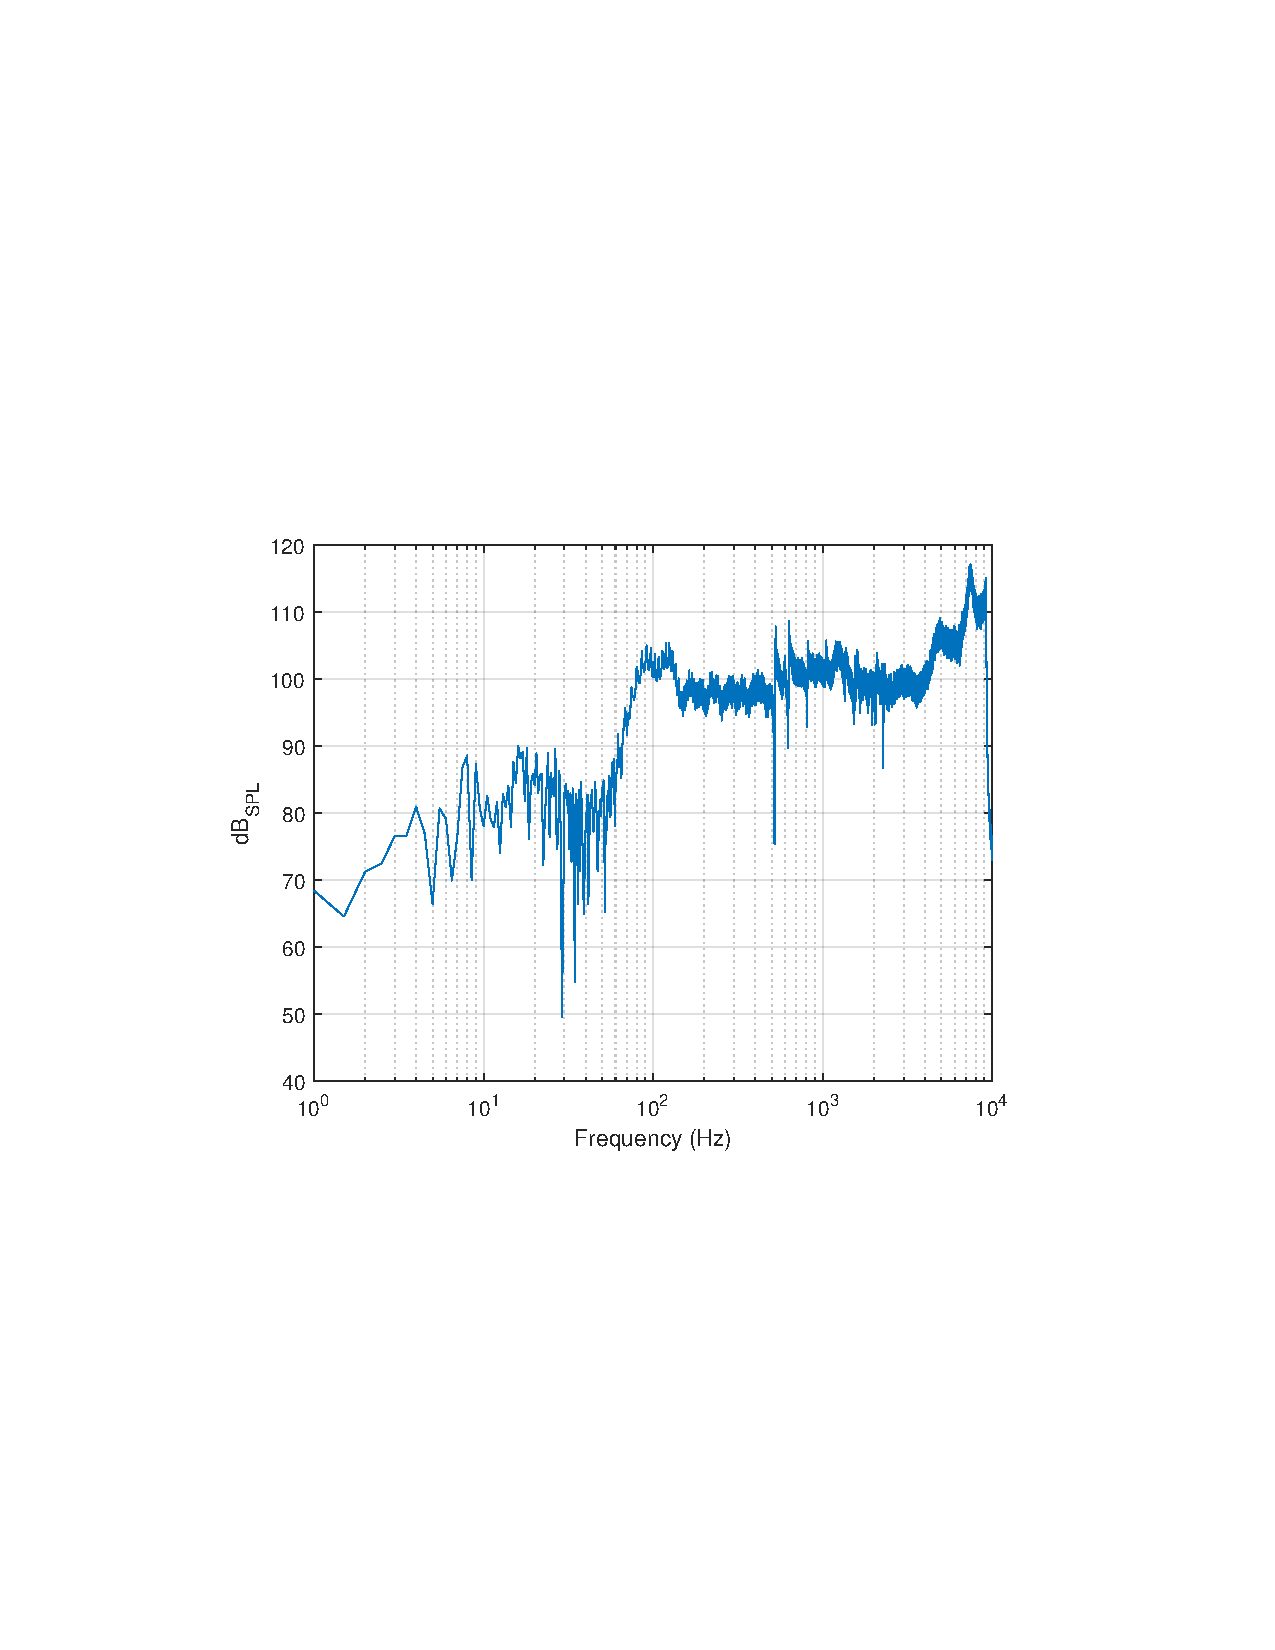
\includegraphics[width=.9\linewidth, clip, trim={3.9cm 8.4cm 4.5cm 9cm}]{gfx/SpeakerMeas/PGopen.pdf}
		\caption{See-through speaker. Bottom opening open.}
		\label{fig:measPGopen}
	\end{subfigure}
	\\
	\begin{subfigure}[t]{.5\textwidth}
		\centering
		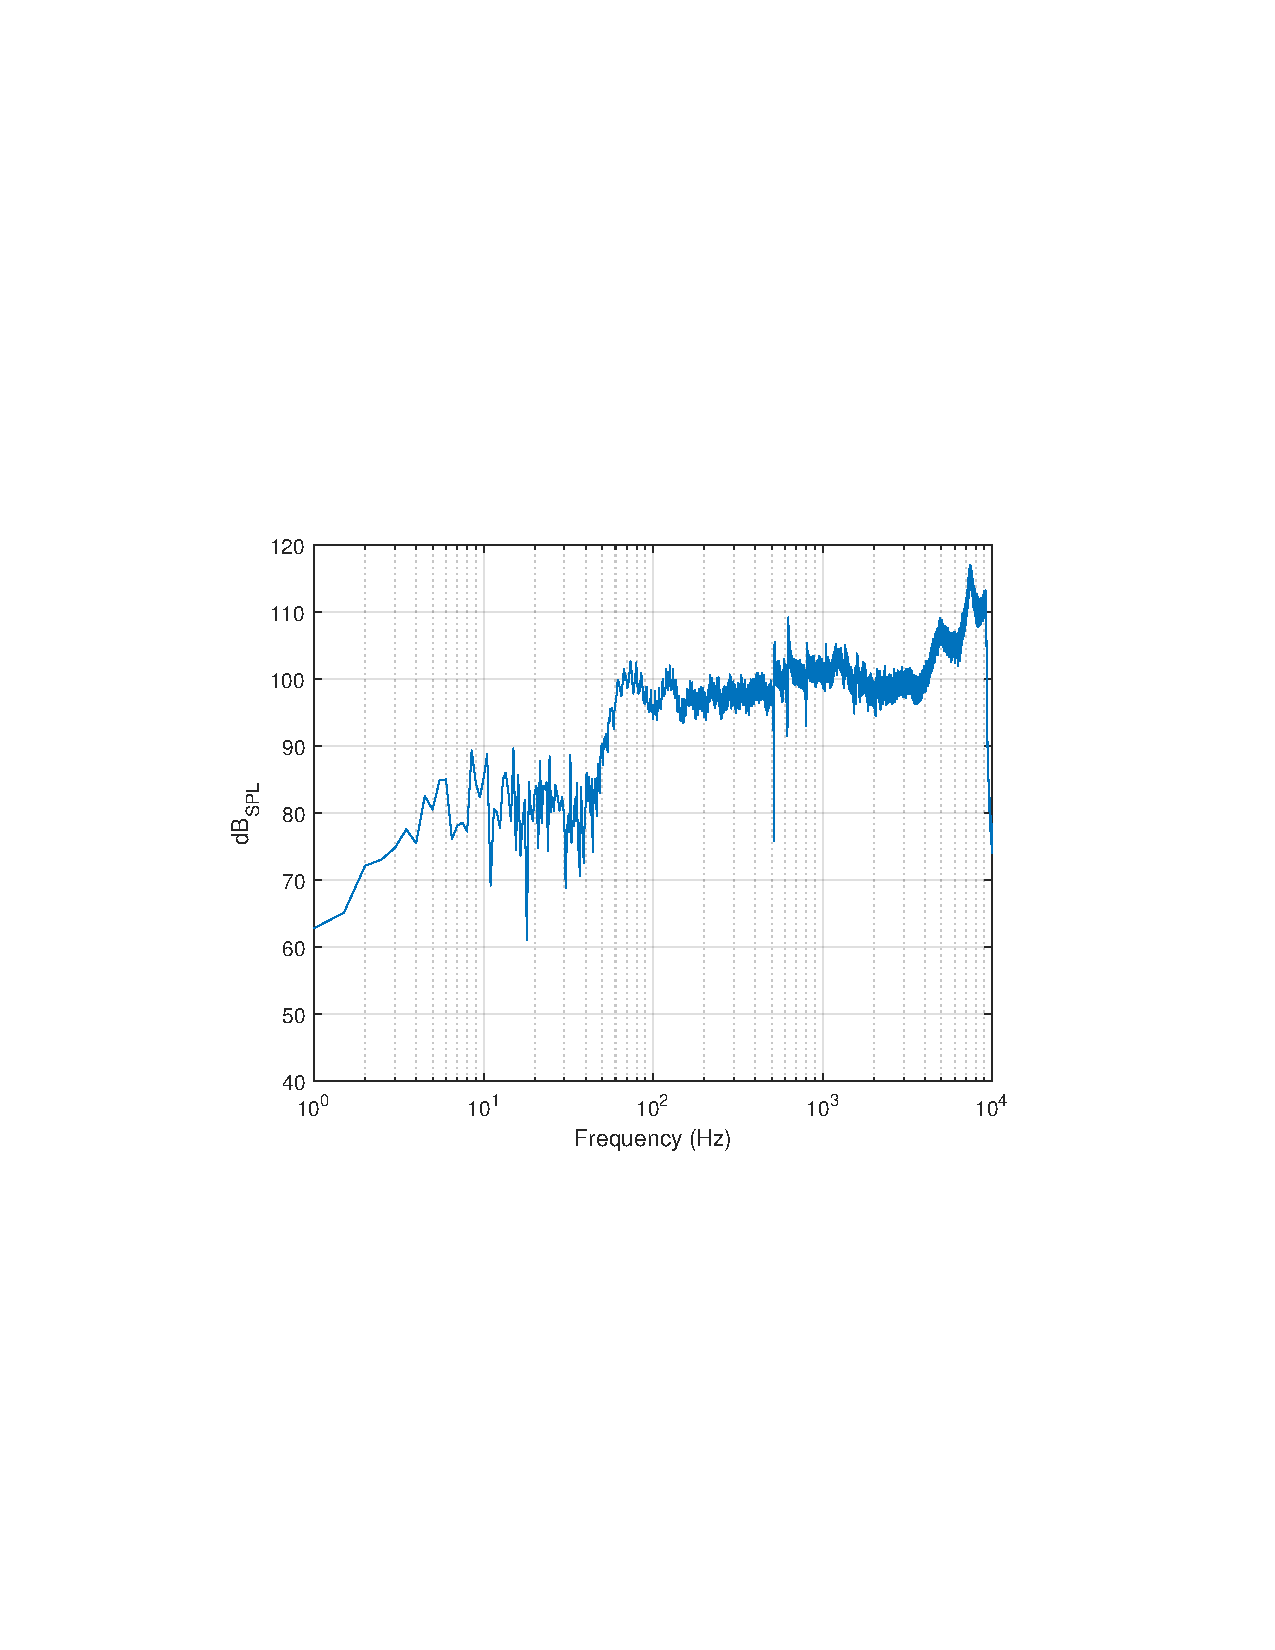
\includegraphics[width=.9\linewidth, clip, trim={3.9cm 8.4cm 4.5cm 9cm}]{gfx/SpeakerMeas/PGBR.pdf}
		\caption{See-through speaker. Bass reflex with length \SI{7}{\centi\metre} and diameter \SI{5}{\centi\metre} inserted at bottom.}
		\label{fig:measPGbass}
	\end{subfigure}%
	\begin{subfigure}[t]{.5\textwidth}
		\centering
		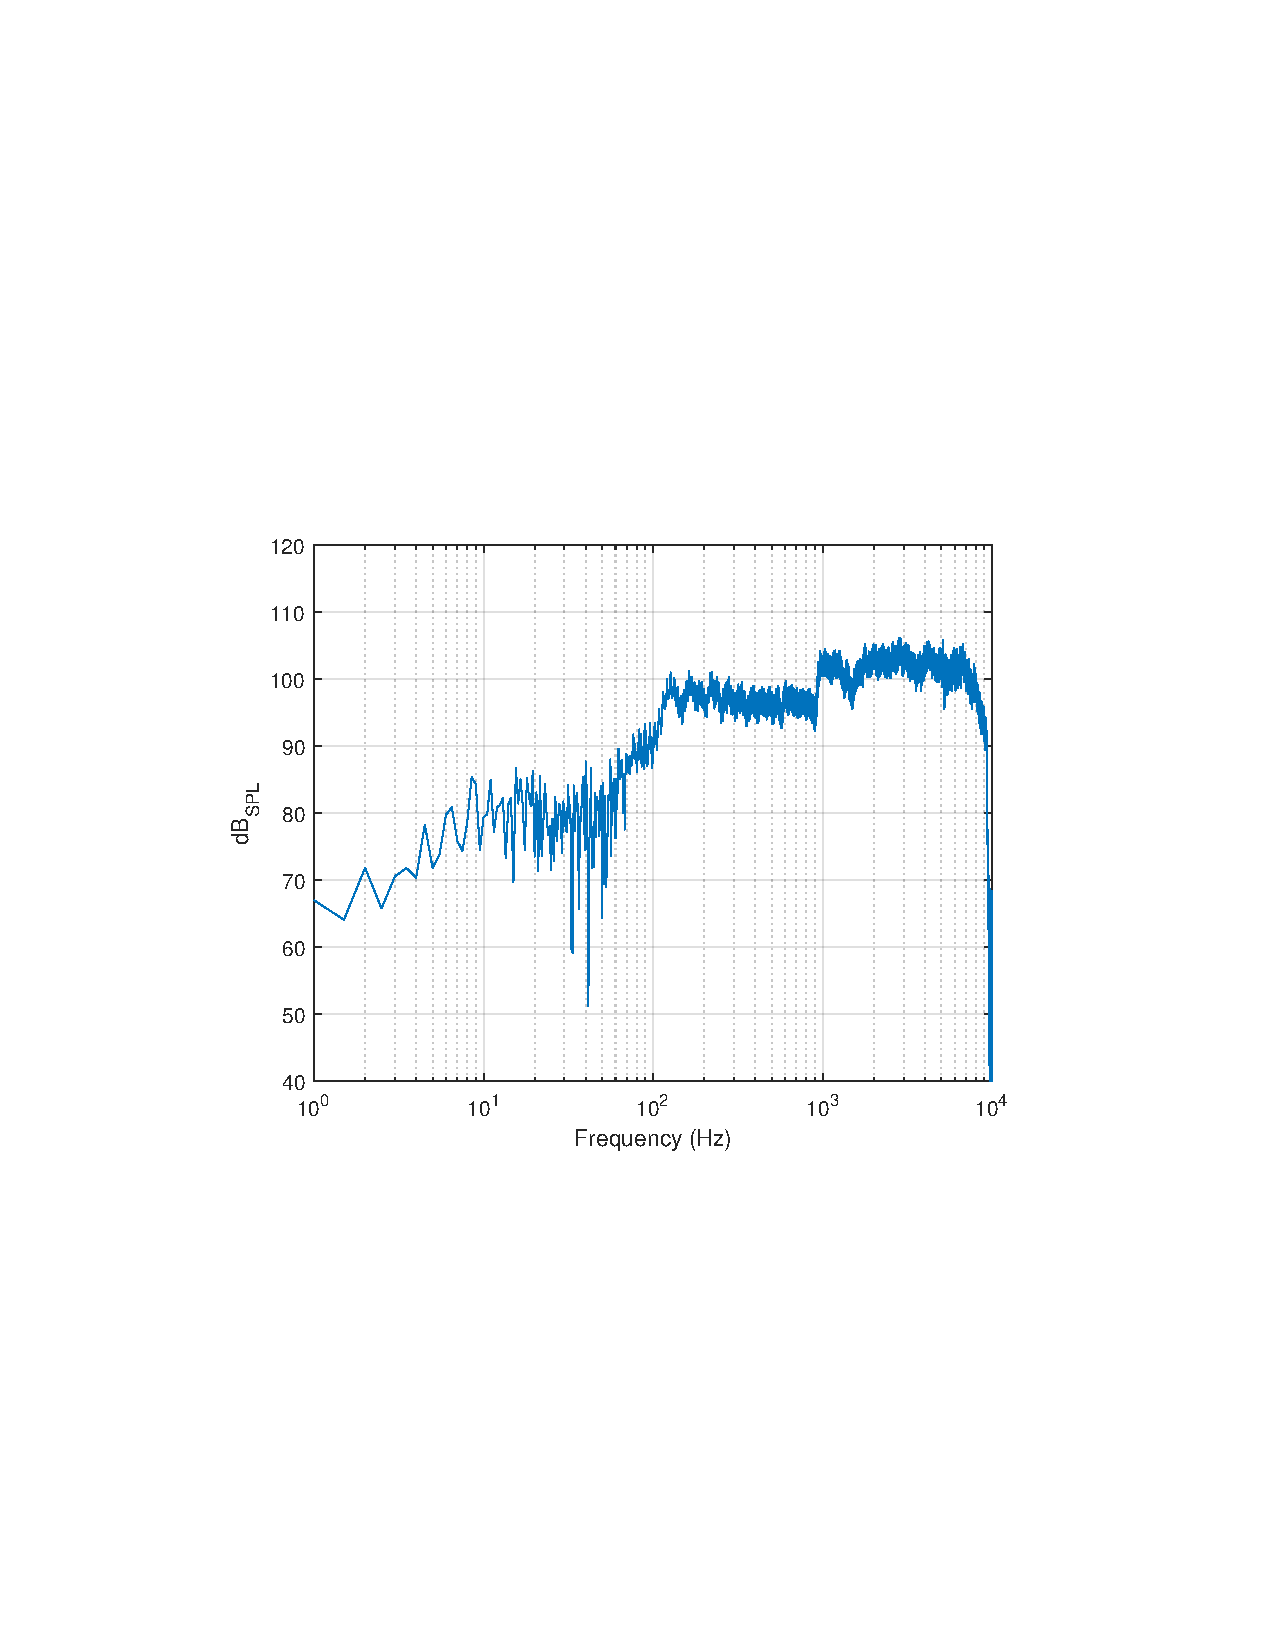
\includegraphics[width=.9\linewidth, clip, trim={3.9cm 8.4cm 4.5cm 9cm}]{gfx/SpeakerMeas/PKclosed.pdf}
		\caption{Wooden speaker measurement.}
		\label{fig:measPK}
	\end{subfigure}
	\caption{Measurements of the speakers.}
	\label{fig:measAll}
\end{figure}

Comparing the closed box approach of both speakers, \cref{fig:closedcompare}, they differ mostly in the regions \SIrange{50}{100}{\hertz} and \SIrange{400}{10000}{\hertz}.
This is most likely due to different Thiele/Small parameters.

\begin{figure}
	\centering
	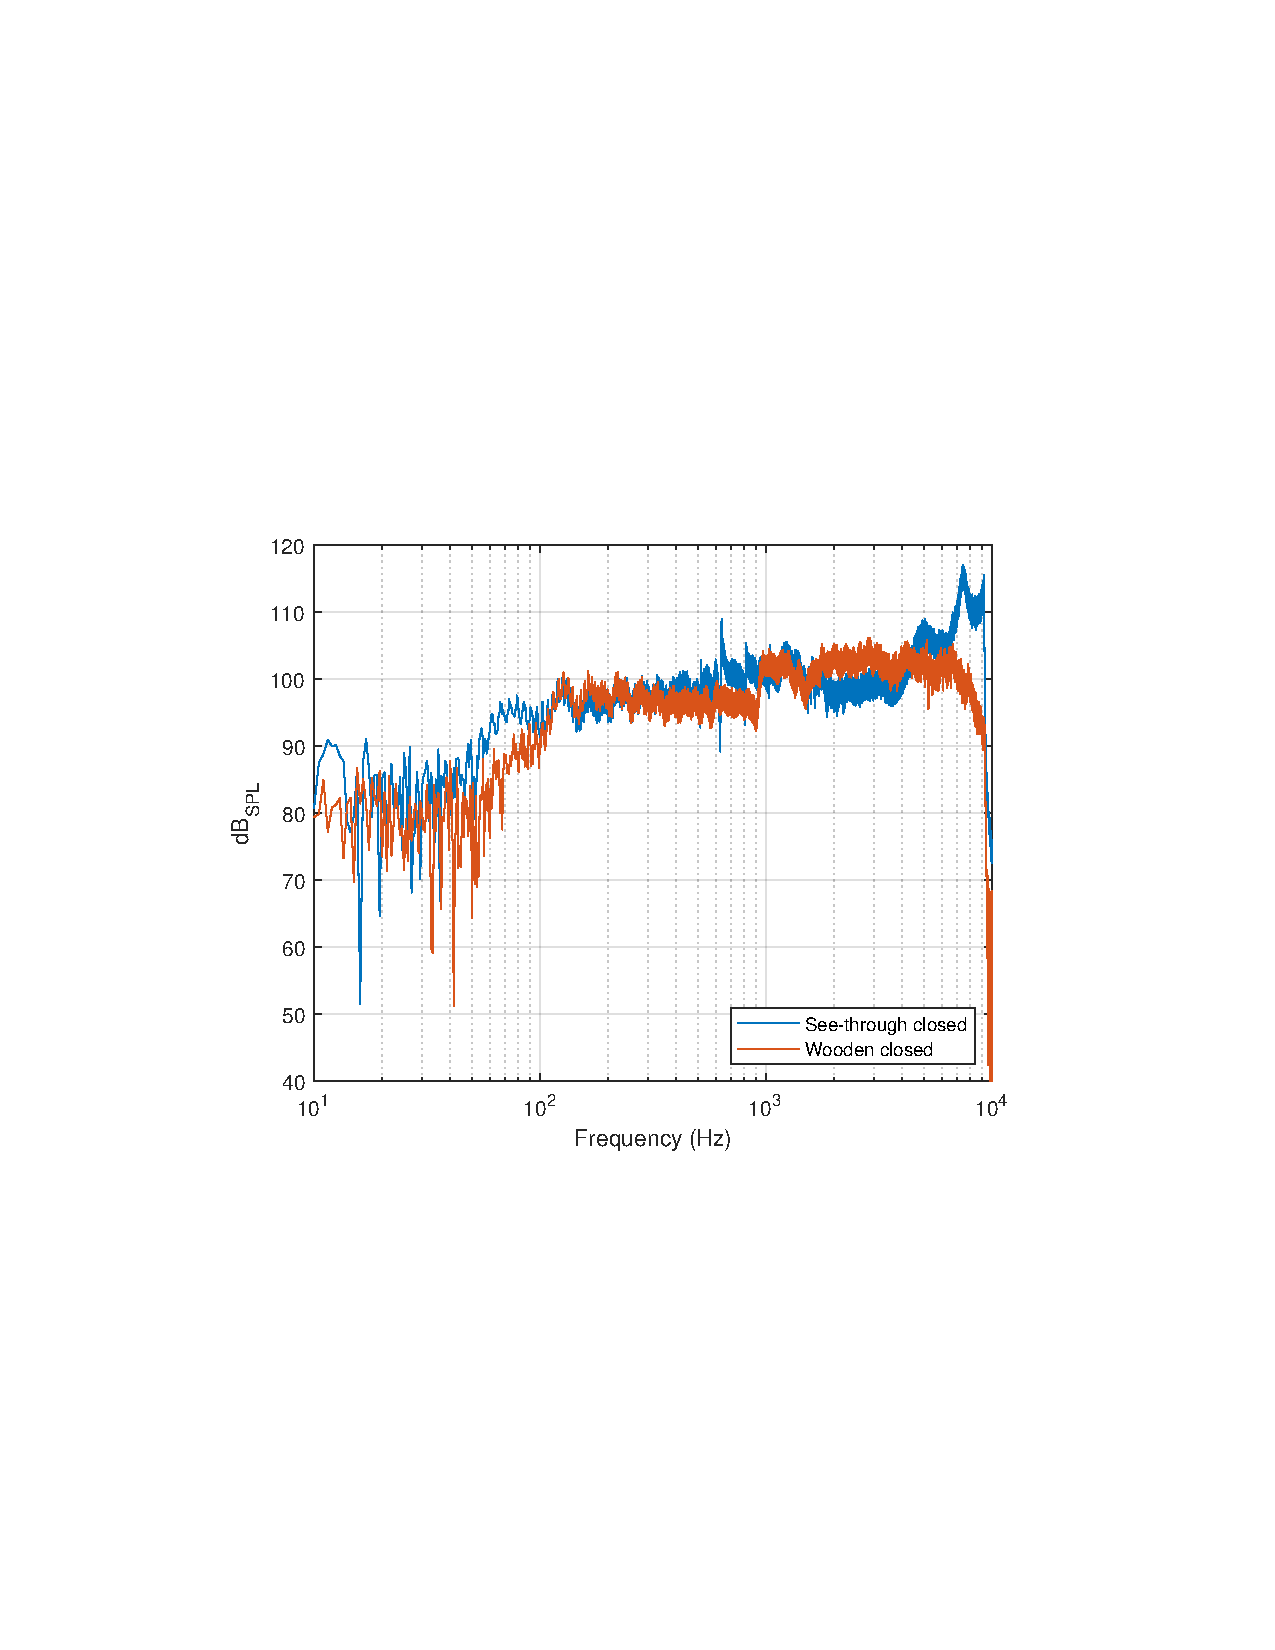
\includegraphics[width=0.7\linewidth, clip, trim={3.9cm 8.4cm 4.5cm 9cm}]{gfx/SpeakerMeas/ClosedCompare.pdf}
	\caption{Comparison of see-through closed and wooden.}
	\label{fig:closedcompare}
\end{figure}

When comparing the see-through speaker setups, \cref{fig:PGcompareAll}, the responses are very similar, except for in the range \SIrange{50}{150}{\hertz}, \cref{fig:PGcompareZoom}.
This is the range at which the response goes from a slope of \SI{12}{\decibel}/octave for the closed setup, and \SI{24}{\decibel}/octave for the open and bass reflex setups, to a more linear frequency response.
Here the gain from using a bass reflex gives approximately \SIrange{3}{5}{\decibel} in the range \SIrange{60}{90}{\hertz}.

\begin{figure}
	\centering
	\begin{subfigure}{.5\textwidth}
		\centering
		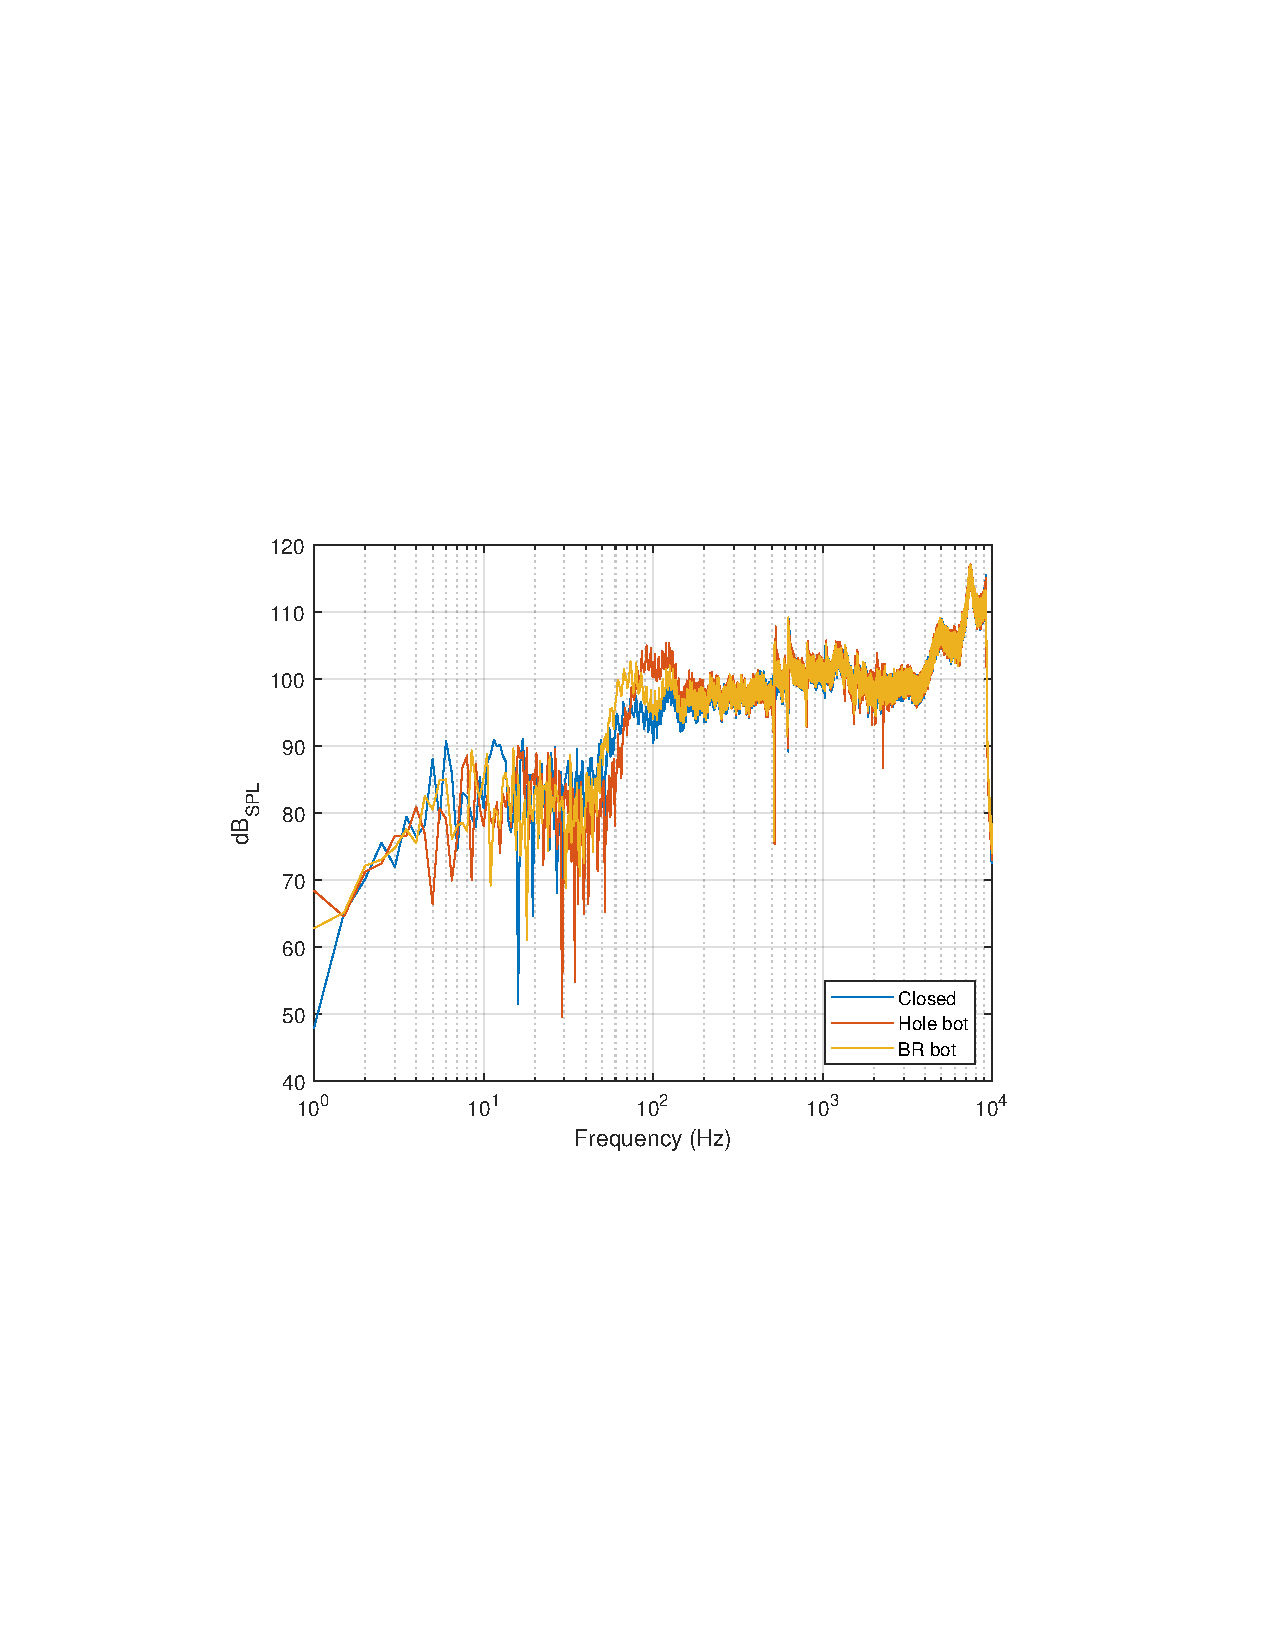
\includegraphics[width=.9\linewidth, clip, trim={3.9cm 8.4cm 4.5cm 9cm}]{gfx/SpeakerMeas/PGcompare.pdf}
		\caption{See-through speaker.}
		\label{fig:PGcompareAll}
	\end{subfigure}%
	\begin{subfigure}{.5\textwidth}
		\centering
		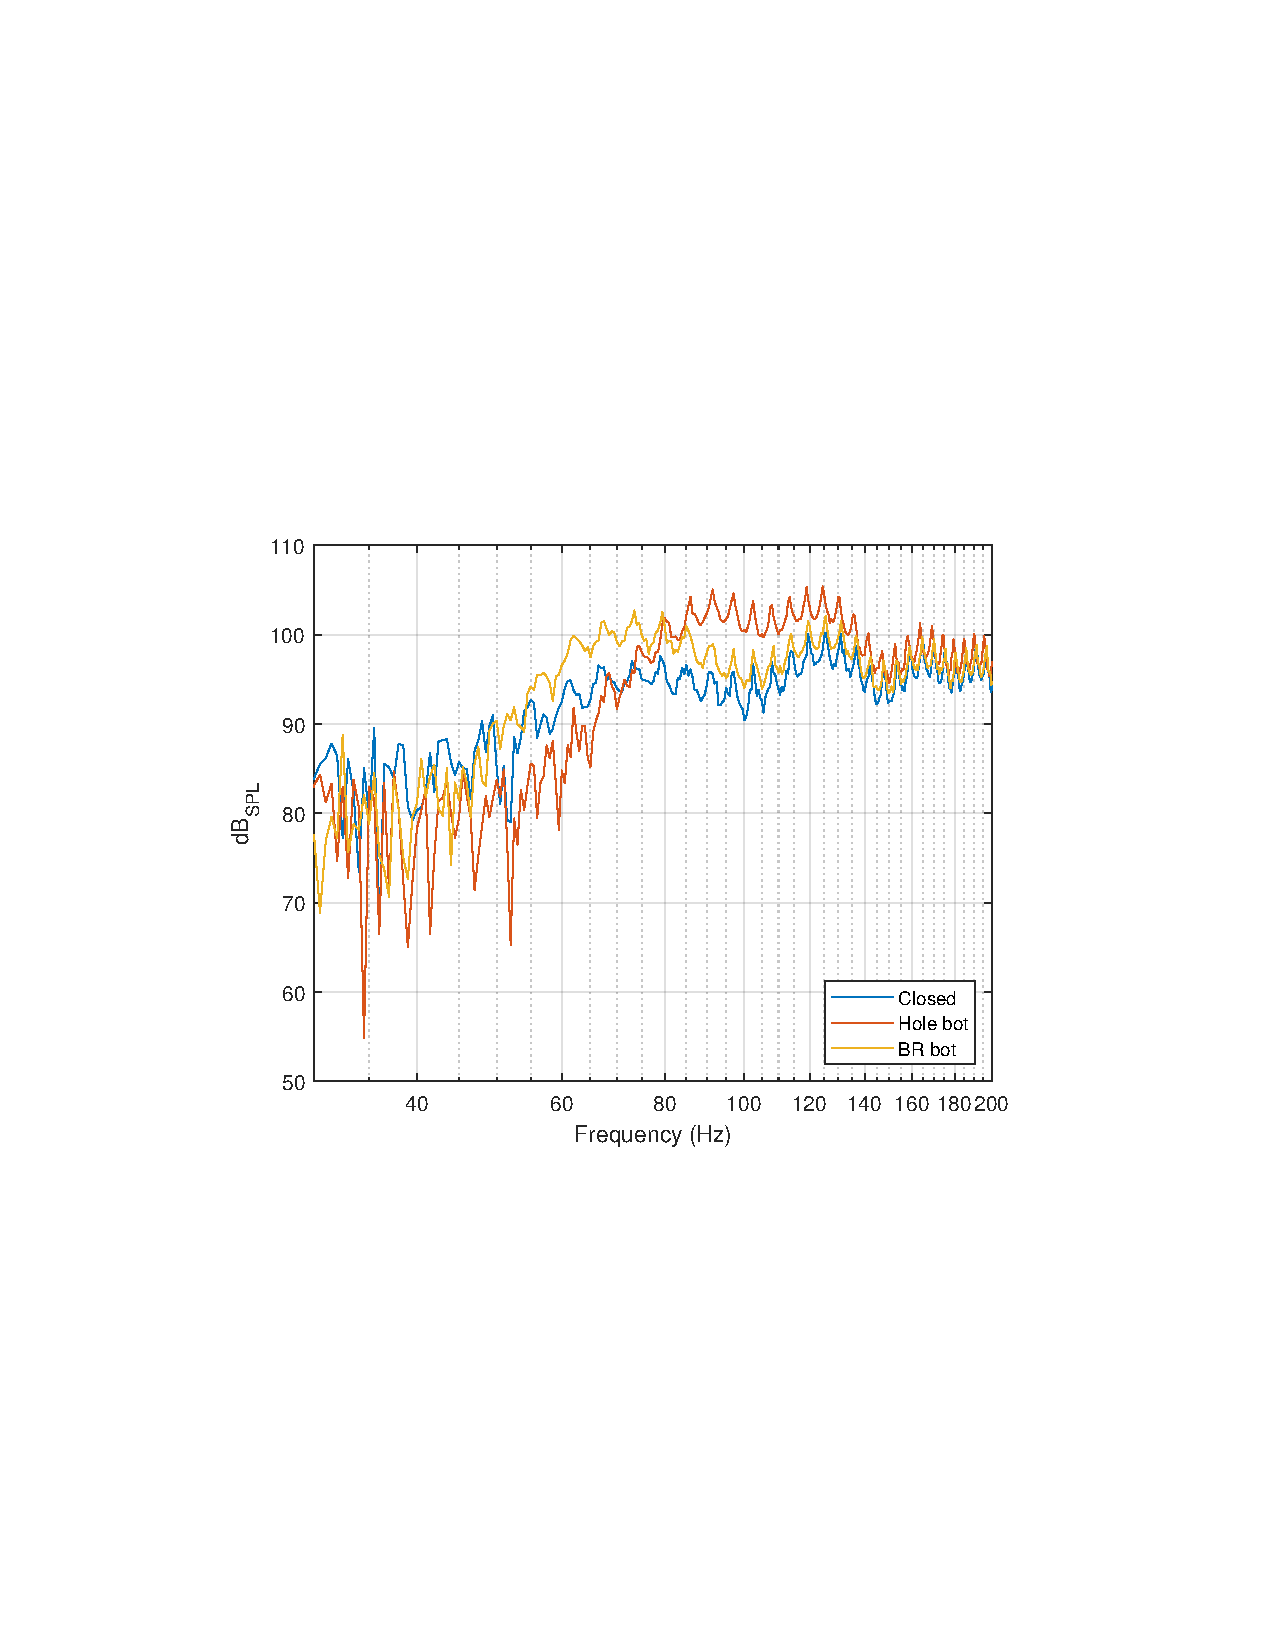
\includegraphics[width=.9\linewidth, clip, trim={3.9cm 8.4cm 4.5cm 9cm}]{gfx/SpeakerMeas/PGcompareZoom.pdf}
		\caption{Zoom of \cref{fig:PGcompareAll}.}
		\label{fig:PGcompareZoom}
	\end{subfigure}
	\caption{Comparison of the different setups of the see-through speaker.}
	\label{fig:PGcompare}
\end{figure}

\FloatBarrier